
\documentclass[a4paper,11pt,oneside]{book}
\usepackage[utf8]{inputenc}
\usepackage[english]{babel}
\usepackage{amsfonts}
\usepackage{amsmath}
\usepackage{amssymb,amsmath,color}
\usepackage{cite}
\usepackage{graphicx}
\usepackage{float}
\usepackage{listings}
\usepackage{hyperref}


\usepackage[a4paper,
            left=2.0cm,
            right=2.0cm,
            top=2.5cm,
            bottom=2.5cm]{geometry}


\begin{document}
\pagestyle{myheadings}

\thispagestyle{empty}                                                 
\begin{center}                                                            
    \vspace{5mm}
    {\LARGE UNIVERSIT\`A DI BOLOGNA} \\                       
      \vspace{5mm}
\end{center}
\begin{center}
  
\includegraphics[scale=.27]{figs/logo_unibo}
\end{center}
\begin{center}
      \vspace{5mm}
      {\LARGE School of Engineering} \\
        \vspace{3mm}
      {\Large Master's Degree in Computer Engineering} \\
      \vspace{20mm}
      {\LARGE Master Thesis Project at European Space Agency} \\
      \vspace{5mm}{\Large\textbf{Sensor Trade-Off with Extended Kalman Filter optimization for Relative Navigation with Floating Satellite Simulator REACSA}}                  
      \vspace{15mm}
\end{center}
\begin{flushleft}                                                                              
     {\large Advisor: \textbf{\@ Prof. Giuseppe Notarstefano}} \\        
     \vspace{3mm}
     {\large Co-advisor: \textbf{\@ Ing. Andrea Drudi}} \\        
     \vspace{13mm}
\end{flushleft}
\begin{flushright}
      {\large Student:}\\
      \vspace{3mm}
      \textbf{\@ Francesca Bocconcelli}
\end{flushright}        %capoverso allineato a destra
\begin{center}
\vfill
      {\large Academic year \@2024/2025} \\
\end{center}



\newpage
\thispagestyle{empty}


\begin{center}
\chapter*{}
\thispagestyle{empty}
{\Huge \textbf{Abstract}}\\
\vspace{15mm}
\end{center}

\newpage\null\thispagestyle{empty}\newpage

\tableofcontents{}
\newpage\null\thispagestyle{empty}\newpage

\listoffigures                          %crea l'elenco delle figure
%\vspace*{2cm}

\chapter*{Introduction}
\addcontentsline{toc}{chapter}{Introduction}
\section*{Motivations} 

\section*{Contributions}

\newpage\null\thispagestyle{empty}\newpage


%%%%%%%%%% Chapter Title %%%%%%%%%%
\chapter{REACSA control architecture: Mixed Integer MPC with binary and continuous actuation }
Example reference \cite{notarstefano2011containment}

\newpage\null\thispagestyle{empty}\newpage

\chapter{REACSA Architecture}
Example reference \cite{notarstefano2011containment}

\newpage\null\thispagestyle{empty}\newpage

\chapter{Gazebo Simulation Environment for REACSA Relative Navigation}

In this chapter, the setup of the REACSA's sensors within the Gazebo simulation environment is presented. 
\\
The robot is divided into three main modules (see the previous section), and two primary sensors are simulated: a LiDAR and a camera. 
The LiDAR is positioned at a lower level to detect low-lying elements in the environment, while the camera is mounted near the top to provide an overall visual perspective.
\\
For the simulation, the sensor parameters are currently chosen as placeholders for testing purposes. Once the actual hardware is selected, these values should be updated accordingly.

\section{LiDAR Sensor}

The LiDAR is defined as a macro link in the \texttt{xacro} format:

\begin{lstlisting}[basicstyle=\ttfamily\scriptsize]
<xacro:macro name="lidar_link" params="name">
  <link name="${name}">
    <inertial>
      <mass value="0.1"/>
      <origin xyz="0 0 0" rpy="0 0 0"/>
      <inertia ixx="0.000166667" iyy="0.000166667" izz="0.000166667"/>
    </inertial>
    <collision>
      <geometry><box size="0.1 0.1 0.1"/></geometry>
    </collision>
    <visual>
      <geometry><box size="0.1 0.1 0.1"/></geometry>
    </visual>
  </link>
</xacro:macro>
\end{lstlisting}

\noindent The LiDAR sensor is then inserted in Gazebo with basic parameters:

\begin{itemize}
    \item Sensor type: GPU LiDAR
    \item Update rate: 10 Hz
    \item Horizontal scan: 1800 samples over 360°
    \item Vertical scan: 16 samples over ±15°
    \item Range: 0.9 to 100 m (currently reduced for simplicity)
    \item Resolution: 3 cm
\end{itemize}

\begin{lstlisting}[basicstyle=\ttfamily\scriptsize]
<gazebo reference="reacsa_lidar_link">
  <sensor name="lidar_sensor" type="gpu_lidar">
    <topic>lidar</topic>
    <update_rate>10</update_rate>
    <frame>reacsa_lidar_link</frame>
    <lidar>
      <scan>
        <horizontal><samples>1800</samples><min_angle>-3.141593</min_angle><max_angle>3.141593</max_angle></horizontal>
        <vertical><samples>16</samples><min_angle>-0.261799</min_angle><max_angle>0.261799</max_angle></vertical>
      </scan>
      <range><min>0.9</min><max>100</max><resolution>0.03</resolution></range>
    </lidar>
    <alwaysOn>1</alwaysOn>
    <visualize>true</visualize>
  </sensor>
</gazebo>
\end{lstlisting}

\section{Camera Sensor}

The camera is similarly defined as a macro link:

\begin{lstlisting}[basicstyle=\ttfamily\scriptsize]
<xacro:macro name="camera_link" params="name">
  <link name="${name}">
    <inertial><mass value="0.1"/><origin xyz="0 0 0" rpy="0 0 0"/>
      <inertia ixx="0.000166667" iyy="0.000166667" izz="0.000166667"/>
    </inertial>
    <visual><geometry><box size="0.1 0.1 0.1"/></geometry><material name="red"/></visual>
    <collision><geometry><box size="0.1 0.1 0.1"/></geometry></collision>
  </link>
</xacro:macro>
\end{lstlisting}

\noindent In Gazebo, the camera sensor is configured with the following properties:

\begin{itemize}
    \item Sensor type: Camera
    \item Horizontal field of view: 1.047 rad
    \item Image resolution: 320x240 pixels
    \item Clipping range: 0.1–100 m
    \item Update rate: 30 Hz
    \item Visualization enabled
\end{itemize}

\begin{lstlisting}[basicstyle=\ttfamily\scriptsize]
<gazebo reference="camera_link">
  <sensor name="camera_link" type="camera">
    <camera>
      <horizontal_fov>1.047</horizontal_fov>
      <image><width>320</width><height>240</height></image>
      <clip><near>0.1</near><far>100</far></clip>
    </camera>
    <always_on>1</always_on>
    <update_rate>30</update_rate>
    <visualize>true</visualize>
    <topic>camera</topic>
  </sensor>
</gazebo>
\end{lstlisting}

\noindent This setup allows for initial testing of REACSA's perception capabilities in Gazebo, with modular sensor definitions that can be easily replaced once the final hardware is selected.

\newpage\null\thispagestyle{empty}\newpage

\chapter{Object Detection with Intel RealSense D455 Using ArUco Markers}

This chapter presents a method for object detection and pose estimation using the Intel RealSense D455 depth camera and ArUco markers. 
The approach relies on placing fiducial markers on the object of interest to facilitate accurate and robust pose estimation. 
The methodology can be divided into three main stages: creation of ArUco markers, camera calibration, and marker detection with pose estimation.

As part of this project, the implementation is available on GitHub, in the object\_det directory at the following link: 
\href{https://github.com/francy2001/relative_navigation.git}{GitHub Repository}.

\section{Intel RealSense Depth Camera D455}

The Intel\textsuperscript{\textregistered} RealSense\texttrademark\ Depth Camera D455 is a high-performance stereo depth camera that combines precision depth sensing with RGB imaging in a compact form factor. 
Its design allows for rapid integration into robotic platforms, machine vision systems, and industrial applications, making it a versatile tool for both research and development.
\\
The D455 relies on dual global shutter sensors to capture depth information using stereo vision. 
This approach enables accurate distance measurements across a range of 0.4 meters up to approximately 6 meters, depending on ambient lighting conditions. 
The depth sensor provides a resolution of up to $1280 \times 720$ pixels at 90 frames per second, while the integrated RGB sensor can capture images up to $1280 \times 800$ pixels at the same frame rate. 
This combination ensures that both geometric and visual information are available for object detection, mapping, and navigation tasks.
\\
A key feature of the D455 is its wide field of view, which exceeds 90° diagonally, allowing the camera to perceive larger portions of the environment in a single frame. 
Additionally, the camera integrates a 6 Degrees of Freedom (6DoF) Inertial Measurement Unit (IMU), providing complementary motion information that can improve stabilization, tracking, and sensor fusion algorithms.
\\
The camera is powered via a USB 3.1 Gen 1 connection, which simplifies hardware integration by providing both data transfer and power through a single cable. 
Its compact dimensions and lightweight design make it particularly suitable for mobile robots, drones, and embedded vision systems where space and weight constraints are critical.
\\
The D455 is supported by the Intel\textsuperscript{\textregistered} RealSense SDK 2.0, which is compatible with Windows, Linux, and macOS. 
The SDK offers APIs in C++, Python, and other languages, and includes tools for calibration, visualization, and integration with popular frameworks such as ROS, OpenCV, and Unity. 


\section{Object Detection}

\subsection{Creation of ArUco Markers}

To enhance the robustness of pose estimation, multiple ArUco markers are generated and attached to the object. 
The markers are created programmatically and randomly positioned on a virtual board to avoid overlapping positions. 
A sample code snippet for marker generation is shown below:

\begin{lstlisting}[basicstyle=\ttfamily\scriptsize, language=Python]
for i in range(num_markers):
    marker_id = random.randint(0, dictionary.bytesList.shape[0] - 1)
    marker_img = cv2.aruco.generateImageMarker(dictionary, marker_id, marker_size)
    # Random placement logic to avoid overlap
    # Place marker on virtual board
\end{lstlisting}

\noindent After printing, the markers are physically attached to the object to provide detectable reference points for pose estimation.

\subsection{Camera Calibration}

Accurate pose estimation requires precise knowledge of the camera intrinsic parameters. 
Calibration is performed using a standard chessboard pattern, captured in multiple poses. The corners of the chessboard are detected and refined using sub-pixel accuracy:

\begin{lstlisting}[basicstyle=\ttfamily\scriptsize, language=Python]
ret, corners = cv2.findChessboardCorners(gray, chessboard_size, None)
if ret:
    corners = cv2.cornerSubPix(gray, corners, (11, 11), (-1, -1), criteria)
    objpoints.append(objp)
    imgpoints.append(corners)
ret, mtx, dist, rvecs, tvecs = cv2.calibrateCamera(objpoints, imgpoints, gray.shape[::-1], None, None)
\end{lstlisting}

\noindent The resulting intrinsic matrix \texttt{camera\_matrix} and distortion coefficients \texttt{dist\_coeffs} are then used for marker detection and pose estimation.

\subsection{ArUco Marker Detection and Pose Estimation}

With the camera calibrated, ArUco markers are detected in the RGB images captured by the RealSense camera. 
The detection process uses a predefined ArUco dictionary and detector parameters. 
If markers are detected, their individual poses are estimated, and the axes are drawn on the image for visualization:

\begin{lstlisting}[basicstyle=\ttfamily\scriptsize, language=Python]
aruco_dict = aruco.getPredefinedDictionary(aruco_type)
parameters = aruco.DetectorParameters()
detector = aruco.ArucoDetector(aruco_dict, parameters)
corners, ids, rejected = detector.detectMarkers(gray)

if ids is not None:
    rvecs, tvecs, _ = aruco.estimatePoseSingleMarkers(corners, marker_size, mtx, dist)
\end{lstlisting}

\noindent Finally, the overall pose of the object is estimated by fusing the positions and orientations of all detected markers. 
The translation vectors are averaged, and the rotations are converted to quaternions, averaged, normalized, and converted back to rotation vectors:

\begin{lstlisting}[basicstyle=\ttfamily\scriptsize, language=Python]
if len(tvecs) > 0:
    t_fused = np.mean(np.array(tvecs), axis=0)
    quaternions = [R.from_rotvec(r).as_quat() for r in rvecs]
    quat_mean = np.mean(quaternions, axis=0)
    quat_mean /= np.linalg.norm(quat_mean)
    r_fused = R.from_quat(quat_mean).as_rotvec()
\end{lstlisting}

\noindent This fused pose provides a reliable estimate of the object's position and orientation, enabling downstream applications such as robotic manipulation or navigation in structured environments.

\begin{figure}[H]
    \centering
    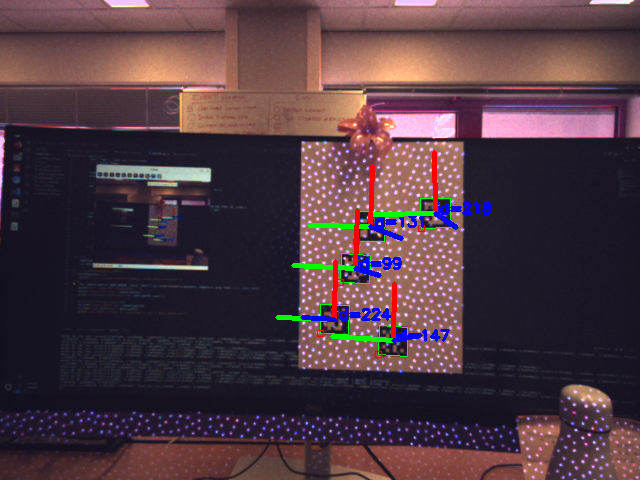
\includegraphics[width=0.6\textwidth]{figs/aruco_det.png}
    \caption{ArUco marker detection and pose estimation visualization.}
    \label{fig:aruco_detection}
\end{figure}
\newpage\null\thispagestyle{empty}\newpage

\chapter{Pose Estimation with 3D Velodyne LiDAR}

This chapter presents a real-time approach for pose estimation using 3D LiDAR data from the Velodyne VLP-16 sensor. 
There will be a description of the sensor, data acquisition, and key processing steps, including ground-plane segmentation, clustering, and state estimation, 
enabling accurate and efficient object tracking in dynamic environments. \\

As part of this project, the implementation is available on GitHub, in the reacsa\_relative\_navigation directory at the following link: 
\href{https://github.com/francy2001/relative_navigation.git}{GitHub Repository}.

\section{Velodyne VLP-16 LiDAR Sensor}

The Velodyne VLP-16 is a compact, cost-efficient 3D LiDAR sensor widely used in robotics, autonomous vehicles, and terrestrial mapping. \\
It integrates 16 infrared (IR) laser/detector pairs within a robust, weather-resistant housing, enabling precise distance measurements to surrounding objects. 
Each laser is fired at a rate of approximately 18.08 kHz, producing up to 300,000 points per second in single return mode and 600,000 points per second in dual return mode. 
The sensor rotates internally to provide a full 360° horizontal scan and a ±15° vertical field of view.

\begin{figure}[H]
    \centering
    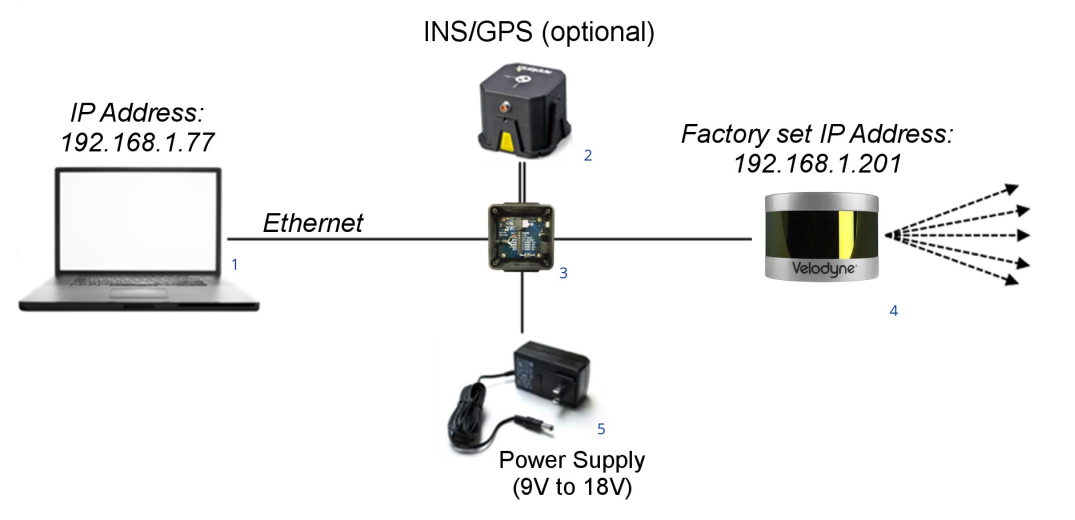
\includegraphics[width=0.7\textwidth]{figs/VELODYNE_1.png}
    \caption{Velodyne VLP-16 Puck Sensor.}
    \label{fig:3DSensingSystem}
\end{figure}

\noindent The VLP-16 operates based on the time-of-flight (ToF) principle. Each emitted IR laser pulse is timestamped and directed in a specific orientation. \\
When the pulse strikes an object, a fraction of its energy is reflected back to the paired detector, which records the return time and intensity. 
This process yields both accurate distance measurements and calibrated reflectivity data, facilitating detection of retro-reflective targets such as street signs, 
license plates, and lane markings.
\\
Its compact footprint, low weight (~830 g), and power efficiency (8 W typical) make it particularly suitable for integration into autonomous systems and robotic platforms.

\subsection{Specifications}
\begin{itemize}
    \item Channels: 16
    \item Measurement Range: 100 m
    \item Range Accuracy: up to ±3 cm (typical)
    \item Vertical Field of View: +15° to -15° (30° total)
    \item Vertical Angular Resolution: 2.0°
    \item Horizontal Field of View: 360°
    \item Horizontal/Azimuth Angular Resolution: 0.1° - 0.4°
    \item Rotation Rate: 5 Hz - 20 Hz
    \item Laser Classification: Class 1 Eye-safe (IEC 60825-1:2007 \& 2014)
    \item Wavelength: 903 nm
    \item Power Supply: 9-18 V (with interface box)
    \item Environmental Protection: IP67
    \item Operating Temperature: -10°C to +60°C
    \item Storage Temperature: -40°C to +105°C
    \item Ethernet Connection: 100 Mbps, UDP packets include time-of-flight, reflectivity, rotation angles, and synchronized timestamps
    \item GPS Integration: Supports $GPRMC$ and $GPGGA$ NMEA sentences (GPS receiver not included)
\end{itemize}

\noindent The VLP-16 represents a balance between performance, cost, and ease of integration, providing real-time 3D point cloud data for advanced perception tasks in mobile and stationary platforms.

\section{Pose Estimation Algorithm with 3D LiDAR}

\subsection{Overview}

A 3D LiDAR (Light Detection and Ranging) sensor actively emits laser pulses and measures the time of flight of returned signals to reconstruct a three-dimensional representation 
of the environment. Each return provides the three spatial coordinates \((x,y,z)\) of a surface point together with an intensity value that reflects surface reflectivity. 
The acquired point cloud provides dense geometric information that is largely invariant to ambient illumination, making LiDAR a robust modality for outdoor scenes. \\

The pipeline presented here takes raw point cloud frames as input and produces tracked object estimates suitable for downstream modules (e.g. motion planning or mapping). 
The main stages are: \begin{enumerate}
    \item preprocessing and data reduction,
    \item ground-plane segmentation,
    \item coordinate transformation,
    \item spatial clustering to obtain object candidates,
    \item geometric bounding and state estimation for tracking.
\end{enumerate}
Each stage is described in the following subsections. For clarity of exposition, from this point onward the entities to be reached will be referred to as \emph{obstacles},
while the remaining free space, which represents the usable area to approach them, will be referred to as \emph{road}.

% -------------------------
\subsection{Implementation choices and constraints}

Since the on-board computer will be a simple Raspberry Pi 5, the implementation is designed to be lightweight and efficient, capable of running in real time on limited computational resources.
\\
The implementation used in this project is written in C++ with a focus on low-latency execution on an embedded platform. 
The design choices made in the implementation reflect a trade-off between computational cost and the level of geometric detail preserved from the raw sensor data. 
Where appropriate, data structures and algorithms that reduce unnecessary data movement and memory allocations are employed to maintain real-time capability. \\

The implementation integrates a set of code-level optimizations aimed at reducing runtime overhead and memory pressure on the target embedded hardware. 
A single KD-tree entity is maintained as a dedicated spatial index: rather than rebuilding the KD-tree from scratch for every incoming frame, the KD-tree instance is updated 
or incrementally rebuilt to reflect the current obstacle point set. \\
Data are represented and processed using contiguous arrays (for example, arrays of floating-point coordinates) instead of heavyweight point-cloud objects, 
which improves cache locality and reduces per-element overhead. Pointer-based access patterns are used to avoid copies when passing large buffers between pipeline stages; 
smart pointers express ownership semantics, using std::unique\_ptr for exclusive ownership and std::shared\_ptr where shared ownership is required. \\ 
Move semantics and the elimination of redundant copy operations are applied throughout the code to prevent unnecessary data duplication. Finally, temporary buffers required by nearest-neighbour searches, 
such as the index buffer used in KD-tree radius queries, are allocated once and reused across queries rather than being reallocated per call, reducing allocation churn and improving runtime determinism.

% -------------------------
\subsection{ROS2 Node creation}

The \texttt{LidarListener} class is implemented as a ROS2 Node responsible for subscribing to LiDAR sensor data, processing it, 
and publishing segmented point clouds. The constructor of the class initializes the node and sets up the communication interfaces as follows:

\begin{itemize}
    \item \textbf{Subscriptions:} 
    \begin{itemize}
        \item \texttt{laser\_sub\_} subscribes to the topic \texttt{/reacsa/scan}, which publishes \texttt{sensor\_msgs::msg} \\ \texttt{::LaserScan} messages. 
        \item \texttt{pc\_sub\_} subscribes to the topic \texttt{/reacsa/velodyne\_points}, which publishes \texttt{sensor\_msgs::msg} \\ \texttt{::PointCloud2} messages. 
    \end{itemize}

    \item \textbf{Publishers:} 
    \begin{itemize}
        \item \texttt{plane\_pub\_} publishes segmented points corresponding to planar surfaces on the topic \texttt{/reacsa}\\\texttt{/plane\_points}.
        \item \texttt{obstacle\_pub\_} publishes points corresponding to the obstacle detected in the scene on the topic \texttt{/reacsa/obstacle\_points}.
    \end{itemize}

\end{itemize}

\noindent This design allows the node to continuously receive LiDAR data, process it in real time to extract planes and obstacles, 
and make the segmented results available to downstream modules, such as tracking, motion planning, or mapping. 
The use of separate publishers for plane and obstacle points ensures a clear separation of semantic classes and facilitates modular processing in the pipeline.


\begin{lstlisting}[basicstyle=\ttfamily\scriptsize][language=C++]
LidarListener::LidarListener() : rclcpp::Node("lidar_pose_estimation")
{
    // Subscribe to the topic publishing LaserScan data from the lidar
    laser_sub_ = this->create_subscription<sensor_msgs::msg::LaserScan>(
        "/reacsa/scan", 
        rclcpp::QoS(rclcpp::KeepLast(10)).best_effort(), 
        std::bind(&LidarListener::laserScanCallback, this, std::placeholders::_1)
    );
    // Subscribe to the topic publishing PointCloud2 data from the lidar
    pc_sub_ = this->create_subscription<sensor_msgs::msg::PointCloud2>(
        "/reacsa/velodyne_points", 
        rclcpp::QoS(rclcpp::KeepLast(10)).best_effort(),
        std::bind(&LidarListener::pointCloudCallback, this, std::placeholders::_1)
    );

    // Publishing the segmented point clouds
    plane_pub_ = this->create_publisher<sensor_msgs::msg::PointCloud2>(
        "/reacsa/plane_points", 
        10
    );
    obstacle_pub_ = this->create_publisher<sensor_msgs::msg::PointCloud2>(
        "/reacsa/obstacle_points", 
        10
    );
}
\end{lstlisting}


\subsection{Preprocessing and downsampling}

Raw point clouds typically contain a large number of points: processing them directly at full density can be prohibitively expensive. 
To reduce data volume while preserving salient geometry, a \textbf{voxel-based downsampling} method is applied. 
The space is partitioned into a regular 3D grid of cubic voxels with side length \(v\). All points that fall within the same voxel are aggregated and replaced by a representative point, commonly the centroid of the voxel's contents:

$$
\mathbf{c}_V = \frac{1}{|P_V|} \sum_{p\in P_V} p,
$$

\noindent where \(P_V\) is the set of points within voxel \(V\) and \(\mathbf{c}_V\) denotes the centroid used in the downsampled cloud.
The chosen voxel resolution controls the trade-off between geometric fidelity and computational cost: in practice the value \(v\) is set according to the expected
point density and the scale of objects to be detected.

\medskip

\noindent Processing can be further focused by defining a spatial region of interest (RoI). The RoI limits the points considered by subsequent stages, 
for example by constraining horizontal field of view, maximum range, or vertical limits relative to the sensor height.  \\
In the current implementation, the RoI is constrained to a horizontal field of view of 270 degrees. 
A possible future extension is the adoption of a full 360-degree field of view, which would allow REACSA to perceive targets independently of its relative orientation.

\subsection{Ground-plane segmentation using RANSAC}

To separate traversable surface points from potential obstacles, the pipeline applies a plane-fitting segmentation to extract the road surface. 
The road is modeled as a plane whose algebraic form is

$$
ax + by + cz + d = 0,
$$

and the distance of a point \(p=(x,y,z)\) to the plane is given by

$$
\mathrm{dist}(p,\mathcal{P}) = \frac{|a x + b y + c z + d|}{\sqrt{a^2 + b^2 + c^2}}.
$$

The segmentation uses a \textbf{RANSAC (RANdom SAmple Consensus)} procedure: repeatedly sample a small subset of points, estimate a candidate plane, and count inliers whose distance 
to the candidate plane is below a threshold. The candidate with the largest inlier set is selected and its inliers are labeled as ground. 
Points not explained by the ground model are retained as obstacle candidates. \\
With this algorithm, we are able to detect obstacles and their positions accurately.

\begin{lstlisting}[basicstyle=\ttfamily\scriptsize][language=C++]
template<typename PointT> std::unordered_set<int> LidarListener::Ransac3d(
                                typename pcl::PointCloud<PointT>::Ptr cloud, 
                                int maxIterations, 
                                float distanceTol)
{
    std::unordered_set<int> inliersResult;
    srand(time(NULL));

    // Creation of a plane for each iteration
    // A plane is defined by the equation Ax + By + Cz + D = 0
    for (int i = 0; i < maxIterations; i++)
    {
        std::unordered_set<int> inliers;

        // Randomly pick three unique points to define the plane
        int ind1, ind2, ind3;
        do { ind1 = rand() % cloud->points.size(); } while(false);
        do { ind2 = rand() % cloud->points.size(); } while(ind2 == ind1);
        do { ind3 = rand() % cloud->points.size(); } while(ind3 == ind1 || ind3 == ind2);

        auto p1 = cloud->points[ind1];
        auto p2 = cloud->points[ind2];
        auto p3 = cloud->points[ind3];

        // Define the plane using the three points
        float A = (p2.y - p1.y)*(p3.z - p1.z) - (p2.z - p1.z)*(p3.y - p1.y);
        float B = (p2.z - p1.z)*(p3.x - p1.x) - (p2.x - p1.x)*(p3.z - p1.z);
        float C = (p2.x - p1.x)*(p3.y - p1.y) - (p2.y - p1.y)*(p3.x - p1.x);
        float D = -(A*p1.x + B*p1.y + C*p1.z);

        // Check if the plane is valid (so that the points are not collinear)
        float denom = std::sqrt(A*A + B*B + C*C);
        if (denom == 0) continue; // denom = 0 implies that the three points are collinear 
                                    // => infinite number of planes passing through them

        // Once computed the plane, let's compute the distance of each point to the plane
        // and check if it is within the distanceTol. If so, we add the point to the inliers set
        // Real segmentation phase
        for (int idx = 0; idx < int(cloud->points.size()); idx++)
        {
            auto pt = cloud->points[idx];
            float dist = std::fabs(A*pt.x + B*pt.y + C*pt.z + D) / denom;

            if (dist < distanceTol)
                inliers.insert(idx);
        }
        // If the number of inliers is greater than the current best, update the result
        if (inliers.size() > inliersResult.size())
            inliersResult = inliers;
    }

    return inliersResult;
}
\end{lstlisting}

\subsection{Coordinate transformation}

In order to highlight the most informative dimension of LiDAR measurements, in the segmentation phase the point cloud can be expressed in a \textbf{spherical-like coordinate system} rather than in the original Cartesian frame. 
This transformation places greater emphasis on the radial distance, which directly encodes the depth of each return with respect to the sensor. 
Depth plays a particularly critical role in 3D perception, as small variations along the radial direction can lead to large discrepancies in the reconstruction of object geometry or spatial extent, whereas angular deviations tend to produce comparatively minor distortions. 
When incorporated into a RANSAC-based procedure, this representation provides a more meaningful basis for evaluating inliers and fitting geometric models, since the algorithm becomes inherently more sensitive to errors and structures aligned along the range dimension. 
As a result, spherical parametrization improves the robustness of plane extraction. \\
The transformation from Cartesian to spherical coordinates used here is:

$$
r = \sqrt{x^2 + y^2 + z^2}, \qquad
\theta = \operatorname{atan2}(y,x), \qquad
\phi = \operatorname{atan2}\left(z,\sqrt{x^2+y^2}\right).
$$


\subsection{Spatial indexing: KD-tree}

A K-Dimensional Tree (KD-tree) is a binary search tree specifically designed for organizing points in a $K$-dimensional space. 
It constitutes a space-partitioning data structure in which each node stores a $K$-dimensional point and recursively divides the 
space into two half-spaces. Non-leaf nodes define splitting hyperplanes, with points on the left side of the hyperplane associated 
to the left subtree and points on the right side associated to the right subtree.  
\\
For instance, in a two-dimensional KD-tree, the root node typically splits the space with an axis-aligned vertical line (x-axis), 
its children split the space with horizontal lines (y-axis), and the alternation continues recursively with depth: odd levels 
correspond to x-aligned divisions and even levels to y-aligned divisions. More generally, if we denote the splitting planes 
as $0, 1, \dots, K-1$, the node at depth $D$ splits along dimension $A$, where

\[
    A = D \bmod K.
\]

\noindent Thus, if a node is aligned with plane $A$, all points whose coordinate in that dimension is smaller than the node's value fall 
into the left subtree, while all points with greater or equal coordinates fall into the right subtree.  
\\
The advantage of the KD-tree lies in its efficiency for nearest-neighbor queries. While a naive search in an unstructured dataset 
requires $O(n)$ operations, the KD-tree narrows down the search space to relevant regions, achieving an average complexity of 
$O(\log n)$. This reduction in complexity is possible because points are hierarchically grouped into regions, thereby avoiding 
expensive distance computations with potentially thousands of candidates.  
\\
Once points are inserted into the tree, it becomes possible to perform efficient nearest-neighbor searches. Given a target point, 
the search procedure considers only points within a distance tolerance $\epsilon$. To determine whether a node should be further 
explored, a bounding box centered at the target point with side length $2 \cdot \epsilon$ is defined. If the node lies outside 
this bounding region, it can be discarded without further computation. If the node lies within the bounding box, then the Euclidean 
distance is explicitly computed to verify whether the point should be added to the set of neighbors.  
\\
Additionally, the recursive traversal of the KD-tree further reduces computations. If the bounding box does not intersect the 
splitting hyperplane at a given node, the subtree on the opposite side can be skipped entirely. If, however, the bounding box 
crosses the hyperplane, both subtrees must be explored to ensure correctness.  
\\
In summary, the KD-tree provides an elegant mechanism for spatial data partitioning, supporting efficient nearest-neighbor search 
by drastically reducing the number of candidate points that require explicit distance evaluation. Its logarithmic search time and 
ability to scale to higher-dimensional data make it particularly well suited for applications in point cloud processing, where 
fast neighbor queries are fundamental to clustering and segmentation algorithms.
    
\begin{lstlisting}[basicstyle=\ttfamily\scriptsize][language=C++]
struct Node
{
    std::vector<float> point;
    int id;
    Node* left;
    Node* right;

    Node(std::vector<float> arr, int setId)
    :	point(arr), id(setId), left(NULL), right(NULL)
    {}

    ~Node()
    {
        delete left;
        delete right;
    }
};


struct KdTree
{
    Node* root;
    int idx;
    KdTree()
    : root(NULL)
    {}

    ~KdTree()
    {
        delete root;
    }

    // either use return or use a double pointer/pointer by reference. 
    // using the latter methods, the changes are directly reflected in the calling function
    void insertRec(Node** root, const std::vector<float>& point, int depth, int id)
    {
        if (*root == NULL)
        {
            *root = new Node(point, id);
        }
        else
        {
            int idx = depth % 3;  // Cycles through dimensions 0, 1, 2 (x, y, z)
            if (point[idx] < ((*root)->point[idx]))
                insertRec(&((*root)->left), point, depth + 1, id);
            else
                insertRec(&((*root)->right), point, depth + 1, id);
        }
    }

    void insert(std::vector<float> point, int id)
    {
        // TODO: Fill in this function to insert a new point into the tree
        // the function should create a new node and place correctly with in the root 
        insertRec(&root, point, 0, id);
    }

    // return a list of point ids in the tree that are within distance of target
    bool distCompare(const std::vector<float>& point1, const std::vector<float>& point2, 
                        float distTol)
    {
        // Ensure both points have at least 3 dimensions
        if (point1.size() < 3 || point2.size() < 3) {
            return false;
        }
        
        float x = point1[0] - point2[0];
        float y = point1[1] - point2[1];
        float z = point1[2] - point2[2];
        
        float distSquared = x * x + y * y + z * z;
        return distSquared <= (distTol * distTol);
    }

    void searchRec(const std::vector<float>& target, Node* root, int depth, float distTol, 
                    std::vector<int>& ids)
    {
        if (root != NULL)
        {	
            // 3D bounding box check
            if((root->point[0] >= (target[0] - distTol) && 
            root->point[0] <= (target[0] + distTol)) && 
            (root->point[1] >= (target[1] - distTol) && 
            root->point[1] <= (target[1] + distTol)) &&
            (root->point[2] >= (target[2] - distTol) && 
            root->point[2] <= (target[2] + distTol))) {
                
                if (distCompare(target, root->point, distTol))
                {
                    ids.push_back(root->id);
                }
            }

            int idx = depth % 3;  // Cycles through x, y, z dimensions
            
            if ((target[idx] - distTol) < root->point[idx])
                searchRec(target, root->left, depth + 1, distTol, ids);

            if ((target[idx] + distTol) > root->point[idx])
                searchRec(target, root->right, depth + 1, distTol, ids);
        }
    }

    std::vector<int> search(std::vector<float> target, float distanceTol)
    {
        std::vector<int> ids;
        searchRec(target, root, 0, distanceTol, ids);
        return ids;
    }
};
\end{lstlisting}

\subsection{Euclidean clustering}

Clustering is the process of grouping points in a dataset such that points within the same group (cluster) are spatially close to each other. 
In the context of point cloud processing, one widely adopted approach is \textit{Euclidean clustering}. 
The idea is to form associations between points depending on their Euclidean distance. 
To efficiently perform nearest-neighbor searches required for clustering, the spatial indexing data structure KD-tree is employed.  
\\
The algorithm proceeds as follows:
\begin{enumerate}
    \item Iterate through all points in the point cloud, maintaining a record of which points have already been processed.
    \item For each unprocessed point, initialize a new cluster and add the point to it.
    \item Using the KD-tree, query all points that lie within a predefined distance tolerance from the current point.
    \item For each neighboring point not yet processed, add it to the cluster and recursively expand the search by applying the same proximity query.
    \item Once no more neighbors are found, the current cluster is complete. The algorithm then resumes from the next unprocessed point to start forming a new cluster.
    \item When all points in the dataset have been processed, the algorithm returns a set of clusters, each representing a distinct object or region in the scene.
\end{enumerate}

\noindent This approach is particularly useful for object-level understanding of a scene. 
For instance, after separating the ground plane via segmentation, Euclidean clustering can be applied to the remaining points to distinguish individual objects (in this scenario, the target to reach).

\begin{table}[H]
\centering
\begin{tabular}{|l|l|l|}
\hline
\textbf{Aspect}   & \textbf{Segmentation} & \textbf{Clustering} \\ \hline
\textbf{Goal}     & Divide the data 
                  & Group points based on spatial proximity \\ \hline
\textbf{Example Use} & Separate obstacles 
                     & Identify and label individual objects \\ \hline
\textbf{How}      & Model fitting (RANSAC) 
                  & Euclidean distance thresholding \\ \hline
\textbf{Result}   & Logical separation 
                  & Object-level separation \\ \hline
\textbf{Output}   & Typically 2 groups: inliers vs. outliers 
                  & Multiple groups (clusters) \\ \hline
\end{tabular}
\caption{Comparison between segmentation and clustering approaches in point cloud processing.}
\end{table}

\subsection{Geometric bounding and state estimation}

For each cluster, a geometric bounding representation is computed to summarize the object's spatial extent. Typical representations are axis-aligned or oriented bounding boxes; 
either representation yields a compact description consisting of a centroid, an extent, and an orientation.
\\
To produce a temporally consistent set of object tracks, the pipeline associates successive detections over time and estimates their motion. 
A linear state-space estimator is used to smooth measurements and provide short-term prediction of object position and velocity. 
The estimator operates on a state vector comprising position and velocity components and follows the standard predict-update cycle associated with linear recursive estimators.

\subsection{Results}

In the figures below \ref{fig:results}, the left panel \ref{fig:clustering} shows the result of the clustering process. The red points represent the planar background, 
simulating the floating surface of the laboratory, while the white points correspond to the object, which is initially classified 
as an obstacle and will later be treated as a target to reach. 
The right panel \ref{fig:bbox} illustrates the object with its computed bounding box and includes the initial steps of the Kalman filter 
applied for state estimation, providing a first prediction of the object's position and orientation.


\begin{figure}[H]
    \centering
    \begin{minipage}{0.45\textwidth}
        \centering
        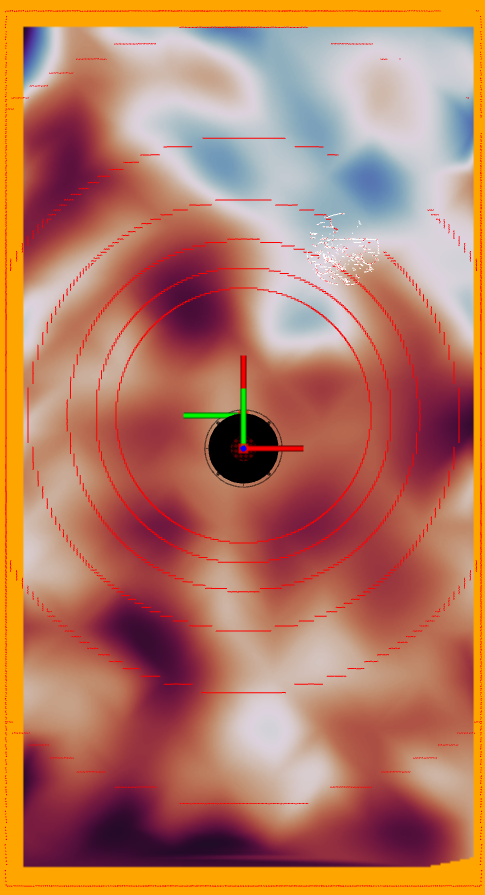
\includegraphics[width=0.8\textwidth]{figs/clustering_results.png}
        \caption{Euclidean Clustering results.}
        \label{fig:clustering}
    \end{minipage}
    \hfill
    \begin{minipage}{0.45\textwidth}
        \centering
        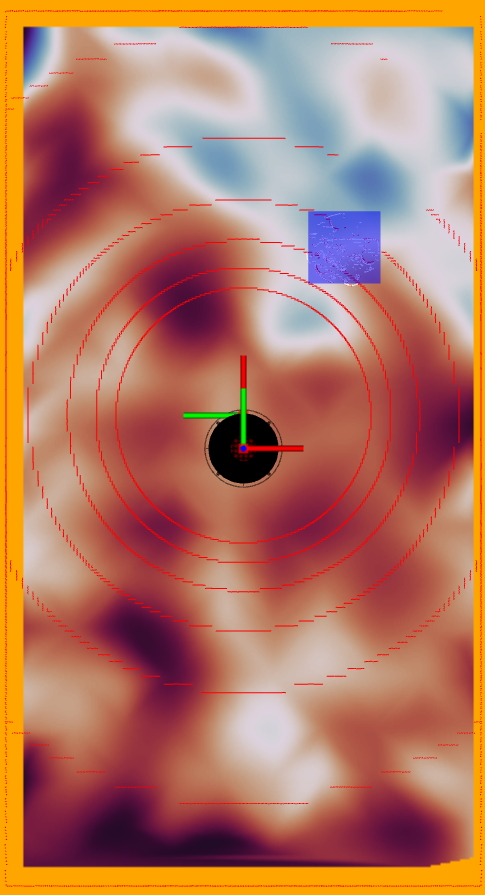
\includegraphics[width=0.8\textwidth]{figs/bbox.png}
        \caption{Bounding box representation for detected object.}
        \label{fig:bbox}
    \end{minipage}
\label{fig:results}
\end{figure}


\newpage\null\thispagestyle{empty}\newpage


\chapter*{Conclusions}
\addcontentsline{toc}{chapter}{Conclusions} 


%%%%%%%%%% Bibliography %%%%%%%%%%%
\bibliography{bibfile}{}
\bibliographystyle{plain}
\addcontentsline{toc}{chapter}{Bibliography}


%%%%%%%%%%%%%%%%%%%%%%%%%%%%%%%%%%%%%%

\end{document}